\subsection{Transformers}
\label{appendix:transformers}

The transformer \cite{transformer} is a model architecture that is based on self-attention mechanism (appendix \ref{appendix:attention}). It is used in many NLP tasks, such as machine translation, text generation, and text classification. The transformer model is composed of an encoder and a decoder: the encoder processes the input sequence, and the decoder generates the output sequence. The transformer model is trained using maximum likelihood estimation (appendix \ref{appendix:likelihood_function}).

In general the transformer can be used for sequence-to-sequence tasks, which is why its so versatile and used in many applications, particularly language tasks, but lately also in image and video synthesis tasks.

\subsubsection{Architecture}

\begin{figure}
    \centering
    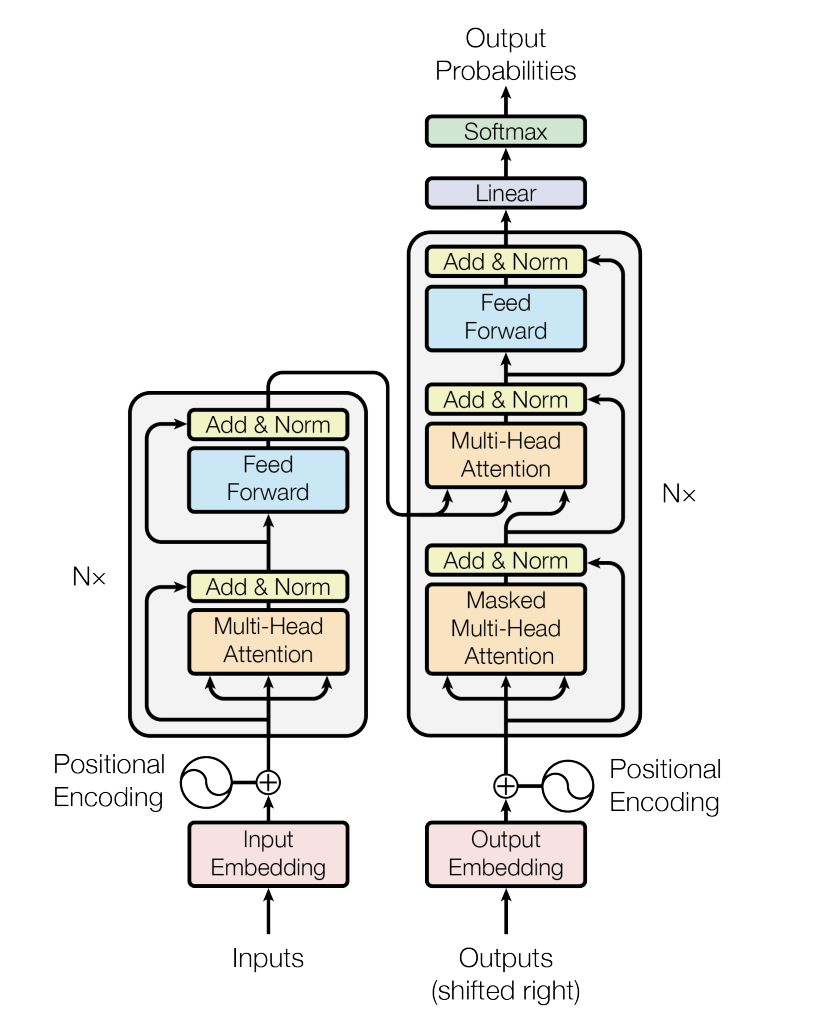
\includegraphics[width=0.5\textwidth]{images/appendix/transformer/architecture.png}
    \caption{Transformer architecture. The encoder (left) processes the input sequence, and the decoder (right) generates the output sequence.}
    \label{fig:appendix_transformer_architecture}
\end{figure}

The architecture overview is shown in figure \ref{fig:appendix_transformer_architecture}.

\textbf{Encoder}: The encoder processes the input sequence and breaks it down to meaningful representations.

\textbf{Decoder}: The decoder takes these representations and generates output sequence autoregressively. 

\subsection*{Encoder}

\textbf{Input}: The input to the encoder (left) is a sequence of tokens (in language tasks). The text is first converted to tokens by a tokenizer. A token is an ID from a vocabulary that will be used. For example, the word "happy" which appears in the vocabulary have the ID of 5, which is a scalar. Some examples of tokenizers include BERT, and T5. After the tokenization, the tokens pass through embedding layer to convert them to a fixed size vector representation (scalar to vector). 

\textbf{Positional embeddings}: Since the transformer has no inherent understanding of sequence or order, positional encodings are added to each embedding to provide information about the position of each token in the sequence. For example the sentence "I am happy" will be tokenized to [12, 8, 5] and then embedded to vectors [[-0.4, 2.1, 0.3], [0.1, 1.2, 0.8], [0.5, 0.2, 0.9]]. The position of the word "I" is 1, "am" is 2, and "happy" is 3. Notice in figure \ref{fig:appendix_transformer_architecture} the positional embeddings are added (element-wise, the dimension stays the same) to the input embeddings before passing them to the encoder. The positional embeddings are computed as sinusoidal functions (sinusoidal embeddings, like we discussed in section \ref{subsec:sinusoidal_embeddings}).

\textbf{Multi-head attention}: The encoder and decoder consists of multiple layers of self-attention and feed-forward neural networks (notice the "Nx" in the diagram, indicating its N blocks). The self-attention mechanism allows the model to weigh the importance of each token in the sequence. The feed-forward neural network processes the output of the self-attention layer. The output of the feed-forward neural network is passed to the next layer. Notice the multi-head attention has 3 inputs, corresponding to the Q,K,V matrices, and all three derive from the same input, indicating its self-attention (unlike cross-attention where the input is projected differently for Q and K,V).

\textbf{Add \& Norm}: After each layer, the output is added to the input (residual connection) and normalized (\texttt{LayerNorm}). This helps the model to learn better and faster (exploding/vanishing gradient problem, whereas normalization layers promoting stability in training; see section \ref{appendix:blocks}).

\subsection*{Decoder}

\textbf{Output embeddings}: The output embeddings are similar to the input embeddings, but they are shifted by one position to the right. This is because the decoder is autoregressive, meaning it generates the output sequence one token at a time. The output embeddings are passed through the positional embeddings, similar to the encoder inputs.

\textbf{Masked multi-head}: The masked multi-head self-attention ensures that the model cannot look at future words in the output sequence during training. Each token can only attend to itself and previous tokens, not the future token (which is why we shift right the output, to generate the next token).

\textbf{Multi-head cross-attention}: The next layer in the decoder is sometimes called "Encoder-Decoder Attention" - it allows the decoder to attend to the output of the encoder (which is projected as K, V), and the output of the previous layer in the decoder (which is projected as Q). In other words, the encoder output is projected in cross-attention as the Q,K matrices, and the decoder outputs shifted right are projected as the V matrix.

\textbf{Linear \& Softmax}: The output of the decoder is passed through a linear layer and a softmax function to generate the probability distribution over the vocabulary. The token with the highest probability is selected as the output token. And the output token is then shifted right and fed back to the decoder as the next input.